\section{Использование коллекций в Windows Forms}
\verb|Задание.| Создать словарь, состоящий из строк. В качестве ключа выступает фамилия, 
в качестве значения — должность. Вывести на экран фамилии людей, занимающих данную должность. 
Вывести должность, занимаемую данным \newline человеком.

Для выполнения данного задания была создана форма, содержащая один элемент \verb|DataGridView|, 
три элемента \verb|Label|, четыре элемента \verb|TextBox| и три элемента \verb|Button| (см. рисунок 
\ref{fig:col_form}). 
\begin{figure}[H]
    \centering
    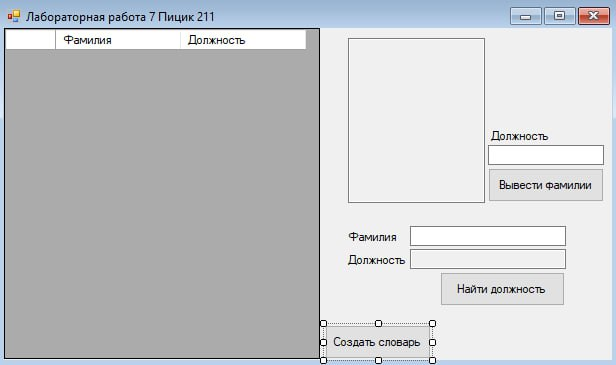
\includegraphics[scale=0.68]{../img/collections/collections_form.png}
    \caption{Вид формы программы обработки отсортированного словаря}
    \label{fig:col_form}
\end{figure}

У элементов формы изменены значения некоторых свойств. С полным списком измененных свойств 
можно ознакомиться в таблице \ref{tab:col_params}.

\begin{table}[H]
    \small
    \caption{Значения атрибутов элементов формы}
    \begin{tabular}{|l|l|}\hline
    Свойство & Значение \cr\hline
    \multicolumn{2}{|l|}{Форма}\cr\hline
    \verb"Text" & Лабораторная Работа 7 Пицик 211 \cr\hline
    \multicolumn{2}{|l|}{Верхняя надпись <<Должность>>}\cr\hline
    \verb"(Name)" & label\_work1 \cr\hline
    \verb"Text" & Должность \cr\hline
    \multicolumn{2}{|l|}{Надпись <<Фамилия>>}\cr\hline
    \verb"(Name)" & label\_surname \cr\hline
    \verb"Text" & Фамилия \cr\hline
    \multicolumn{2}{|l|}{Нижняя надпись <<Должность>>}\cr\hline
    \verb"(Name)" & label\_work \cr\hline
    \verb"Text" & Должность \cr\hline
    \multicolumn{2}{|l|}{Текстовое поле для ввода должности} \cr\hline
    \verb"(Name)" & text\_work1 \cr\hline
    \multicolumn{2}{|l|}{Текстовое поле для вывода фамилий} \cr\hline
    \verb"(Name)" & text\_list \cr\hline
    \verb"ReadOnly" & True \cr\hline
    \verb"Multiline" & True \cr\hline
    \multicolumn{2}{|l|}{Текстовое поле для ввода фамилии} \cr\hline
    \verb"(Name)" & text\_surname \cr\hline
    \multicolumn{2}{|l|}{Текстовое поле для вывода должности} \cr\hline
    \verb"(Name)" & text\_work \cr\hline
    \verb"ReadOnly" & True \cr\hline
    \multicolumn{2}{|l|}{Кнопка <<Создать словарь>>}\cr\hline
    \verb"(Name)" & btn\_dict \cr\hline 
    \verb"Text" & Создать словарь \cr\hline 
    \multicolumn{2}{|l|}{Кнопка <<Вывести фамилии>>}\cr\hline
    \verb"(Name)" & btn\_list\cr\hline
    \verb"Text" & Вывести фамилии \cr\hline
    \multicolumn{2}{|l|}{Кнопка <<Найти должность>>}\cr\hline
    \verb"(Name)" & btn\_find \cr\hline 
    \verb"Text" & Найти должность \cr\hline
    \multicolumn{2}{|l|}{DataGridView для колллекции}\cr\hline
    \verb"(Name)" & dgv\_table\cr\hline
    \verb"AllowUserToAddRows" & False\cr\hline
    \verb"AllowUserToDeleteRows" & False\cr\hline
    \verb"ReadOnly" & True\cr\hline
    \end{tabular}
    \label{tab:col_params}
\end{table}

С помощью свойства \verb|Enabled| элемента \verb|button_dict| осуществляется запрет 
на повторное нажание кнопки \cite{microsoft_enabled}. Создание словаря осуществляется с помощью следующего кода:
\begin{minted}[linenos, breaklines=true, fontsize=\small, style=bw]{cpp}
System::Collections::Generic::SortedDictionary <String^, String^> dict;
\end{minted}
Здесь \verb|dict| "--- название переменной, которое будет иметь отсортированный словарь.
Основные свойства и методы словаря описаны в таблице \ref{tab:col_methods} \cite{microsoft_dict}.

\begin{table}[H]
    \small
    \caption{Свойства и методы словаря}
    \begin{tabular}{|l|l|}\hline
    \multicolumn{2}{|l|}{Свойства}\cr\hline
    \verb"dict.Count()" & возвращает количество элементов словаря \cr\hline
    \verb"dict.Keys()" & возвращает коллекцию, содержащую ключи словаря \cr\hline
    \verb"dict.Values()" & возвращает коллекцию, содержащую значения словаря \cr\hline
    \multicolumn{2}{|l|}{Методы}\cr\hline
    \verb"dict.Clear()" & очистка словаря \cr\hline
    \verb"dict.Add(X)" & добавление нового элемента в словарь \cr\hline
    \verb"dict.ContainsKey(X)" & возвращает \verb|true|, если ключ X есть в словаре \cr\hline
    \verb"dict.ContainsValue(X)" & возвращает \verb|true|, если значение X есть в словаре \cr\hline
    \verb"dict.Remove(X)" & удаляет элемент X \cr\hline
    \verb"dict.TryGetValue(X)" & возвращает \verb|true|, если ключ X есть в словаре и возвращает значение\cr\hline
    \end{tabular}
    \label{tab:col_methods}
\end{table}

Код кнопки <<Создать словарь>> выглядит следующим образом:
\begin{minted}[linenos, breaklines=true, style=bw, fontsize=\small]{cpp}
private: System::Void btn_dict_Click(System::Object^ sender, System::EventArgs^ e) {
    this->btn_dict->Enabled = false;
    System::Collections::Generic::SortedDictionary <String^, String^> dict;
    
    //Элементы словаря
    dict.Add("Пицик", "Старший разработчик");
    dict.Add("Коновалов", "DevOps инженер");
    dict.Add("Дрождев", "Разработчик");
    dict.Add("Цой", "ML-инженер");
    dict.Add("Артамонова", "Средний разработчик");
    dict.Add("Карасёв", "DevOps инженер");
    dict.Add("Воронцов", "Prompt инженер");
    dict.Add("Гришин", "Full-stack разработчик");
    dict.Add("Николаев", "GameDev разработчик");
    dict.Add("Иванов", "Младший разработчик");

    for each (KeyValuePair<String^, String^> item in dict)
    {
      int row = dgv_table->Rows->Add();
      dgv_table->Rows[row]->Cells[0]->Value = item.Key;
      dgv_table->Rows[row]->Cells[1]->Value = item.Value;
    }
  }
\end{minted}
Создаётся словарь \verb|dict|, заполняется с помощью метода \verb|dict.Add()|, а затем 
элементы словаря переносятся в окно элемента \verb|dgv_table| \cite{microsoft_dgv}.
Для корректной работы \verb|KeyValuePair| необходимо разрешить пространство имён \verb|Generic|:
\begin{minted}[linenos, breaklines=true, fontsize=\small, style=bw]{cpp}
using namespace System::Collections::Generic;
\end{minted}

С остальными кодами можно ознакомиться в приложении \ref{app:codes}.

При открытии приложения появляется окно (см. рисунок \ref{fig:cols_res}).
\begin{figure}[H]
  \centering
  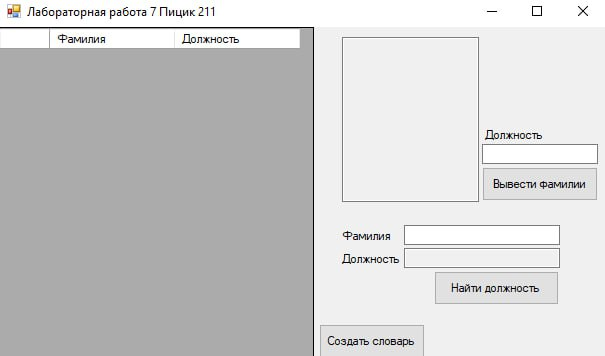
\includegraphics[scale=.85]{../img/collections/collections_res.jpg}
  \caption{Окно приложения <<Коллекции>>: начальный запуск}
  \label{fig:cols_res}
\end{figure}

При нажатии кнопки <<Создать словарь>> обновляется содержимое \newline \verb|DataGidView|
(см. рисунок \ref{fig:cols_create}).
\begin{figure}[H]
  \centering
  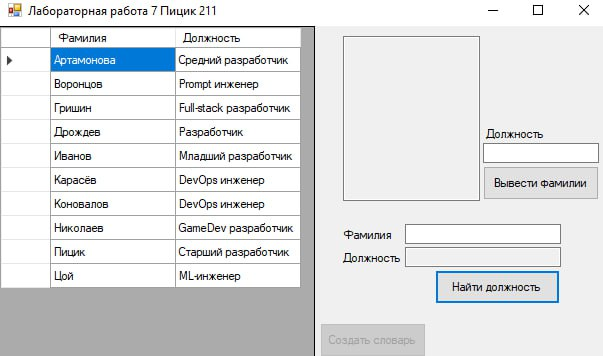
\includegraphics[scale=.85]{../img/collections/collections_create.jpg}
  \caption{<<Коллекции>>: создание словаря}
  \label{fig:cols_create}
\end{figure}

При поиске фамилий по должности или должности по фамилии и корректном вводе данных, 
выводится соответствующий результат как показано на рисунке \ref{fig:cols_find}.
\begin{figure}[H]
  \centering
  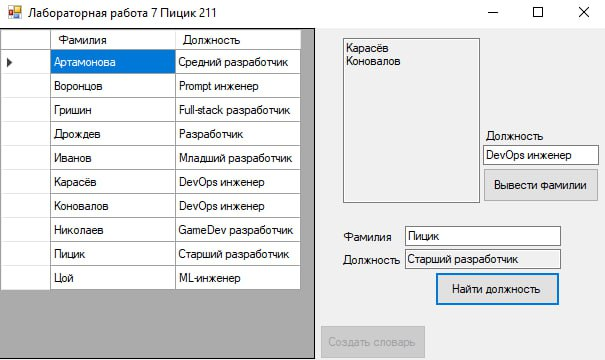
\includegraphics[scale=.85]{../img/collections/collections_find.jpg}
  \caption{<<Коллекции>>: поиск при корректных данных}
  \label{fig:cols_find}
\end{figure}

При поиске с некорректными данными, выводятся соответствующие ошибки 
(см. рисунок \ref{fig:cols_error}).
\begin{figure}[H]
  \centering
  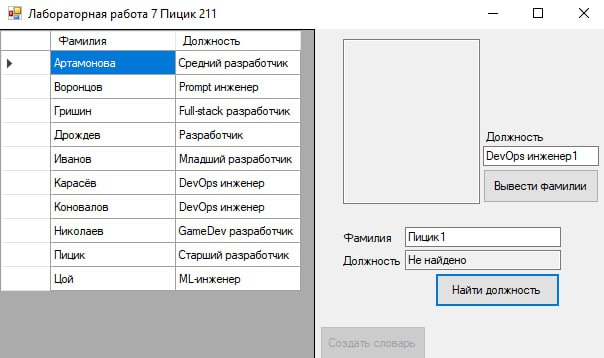
\includegraphics[scale=.85]{../img/collections/collections_error.jpg}
  \caption{<<Коллекции>>: вывод ошибок}
  \label{fig:cols_error}
\end{figure}

Полный код программы доступен в приложении \ref{app:repo}.